%\documentclass[5p,times]{elsarticle}
\documentclass[11pt,review,times]{elsarticle}
%\documentclass[11pt,preprint,times]{elsarticle}

%%%%%%%%%%%%%%%%%%%%%%%%%%%%%%%%%%%%%%%%%%%%%%%%%%%%%%%%%%%%%%%%%
%	Loading packages
%%%%%%%%%%%%%%%%%%%%%%%%%%%%%%%%%%%%%%%%%%%%%%%%%%%%%%%%%%%%%%%%%
\usepackage[english]{babel}
\usepackage[utf8]{inputenc}
\usepackage[T1]{fontenc}
\usepackage{graphicx}
\usepackage{amsfonts}
\usepackage{placeins} % For /Floatbarrier
\usepackage{array,booktabs}
\usepackage{url} % For better linebreaks of URLs
\usepackage{float}

\usepackage[list-units = single,range-units = single]{siunitx}
\sisetup{separate-uncertainty}

\usepackage{caption}
\usepackage{subcaption}
\usepackage{upgreek}
\usepackage[inline]{enumitem}
\usepackage{chemformula}
%\usepackage{mathrsfs}
%\usepackage{wasysym}


% Packages for tikz
\usepackage{tikz}
\usepackage{pgf}
\usepackage{pgfplots}
\usepackage{pgfplotstable}
	\pgfplotstableset{col sep=comma} % call once in your preamble if all your tables use commas as column separator
	\pgfplotstableset{search path={datafiles}} % Put .csv files in /datafiles or the root folder
\usetikzlibrary{3d}
\usetikzlibrary{calc}
\usetikzlibrary{decorations.pathmorphing} % Pour obtenir des lignes de coupes aléatoires
\usetikzlibrary{arrows}
\usetikzlibrary{arrows.meta,shapes,positioning,shadows,trees,decorations.pathmorphing}
\usetikzlibrary{external}
\tikzexternalize[prefix=TikzPictures/]

\biboptions{sort&compress}

\newcolumntype{M}[1]{>{\centering\arraybackslash}m{#1}} % Define a column style "M" (verticaly centered by m) and horizontaly

% Hyperref and parameters of PDF
\usepackage[hidelinks]{hyperref}
\hypersetup{
	pdftitle = {Resistance Welding of Thermoplastic Composites with a Nanocomposite Heating Element},
    pdfauthor = {David Brassard, Martine Dubé, Jason R Tavares},
	pdfkeywords={carbon nanotube, thermal conductivity, polymer, nanocomposite, heating element, Joule heating, electrical conductivity, Finite element analysis, composite, thermoplastic},
	pdfsubject={Resistance Welding of Thermoplastic Composites with a Nanocomposite Heating Element}
}

\graphicspath{{Figures/}}	% Root directory of the pictures 

%%%%%%%%%%%%%%%%%%%%%%%%%%%%%%%%%%%%%%%%%%%%%%%%%%%%%%%%%%%%%%%%%
%	Main document
%%%%%%%%%%%%%%%%%%%%%%%%%%%%%%%%%%%%%%%%%%%%%%%%%%%%%%%%%%%%%%%%%
\begin{document}
\hyphenation{COMSOL na-no-com-po-si-te na-no-com-po-si-tes}


\title{Resistance Welding of Thermoplastic Composites with a Nanocomposite Heating Element}
\journal{Composites Part B: Engineering}

\author[polymtl,crepec]{David~Brassard}
\ead{david.brassard@polymtl.com}
\author[ets,crepec]{Martine~Dubé}
\ead{martine.dube@etsmtl.ca}
\author[polymtl,crepec]{Jason~R.~Tavares\corref{cor1}}
\ead{jason.tavares@polymtl.ca}

\cortext[cor1]{Corresponding author}

\address[polymtl]{Department of Chemical Engineering, Polytechnique Montréal, P.O. Box 6079 Station Centre-Ville, Montréal, QC, H3C 3A7, Canada}
\address[ets]{Department of Mechanical Engineering, École de technologie supérieure, 1100 Notre-Dame Street West, Montréal, Québec, Canada, H3C 1K3}
\address[crepec]{Research Center for High Performance Polymer and Composite Systems (CREPEC), Polytechnique Montréal, P.O. Box 6079 Station Centre-Ville, Montréal, QC, H3C 3A7, Canada}

\begin{abstract}

This work demonstrates, with a multistep approach, that a PEI/MWCNT-based nanocomposite heating element is a viable alternative to stainless steel meshes for resistance welding of high performance thermoplastic composites. 
Simple continuum micromechanic simulations of the nanocomposite predicted uniform temperature at the constituent scale. 
A test with a PEEK/MWCNT nanocomposite heating filament then demonstrated temperature uniformity at the macroscopic scale. 
At the coupon scale, single lap shear specimens with CF/PEEK adherents were welded with the PEI/MWCNT nanocomposite heating element. 
Cohesive failure within the nanocomposite were observed and FTIR tests confirmed the absence of important thermal degradation. 
This nanocomposite heating element offers simplified handling as an intermediate PEI layers is no longer required. 

\end{abstract}

\begin{keyword}
A. Thermoplastic resin;  B. Electrical properties;  B. Mechanical properties;  E. Joints/joining 
\end{keyword}

\maketitle

%%%%%%%%%%%%%%%%%%%%%%%%%%%%%%%%%%%%%%%%%%%%%%%%%%%%%%%%%%%%%%%%%
							\section{Introduction}
%%%%%%%%%%%%%%%%%%%%%%%%%%%%%%%%%%%%%%%%%%%%%%%%%%%%%%%%%%%%%%%%%

The current fierce competition in the space industry is putting a strong downward pressure on the launch cost of satellites. 
New processes and materials are needed to achieve launcher weight and cost reductions. 
Fibre reinforced polymers is a common material used to achieve weight reduction. 
Currently, thermoset polymers are dominating the market of composite matrix but thermoplastic attract the attention of the industry \cite{CompositeWorldSloan2018} for the higher impact resistance, increased production rates, superior recyclability, ability for long-term storage and higher environmental resistance they offer \cite{cogswell1992}. 
Moreover, a distinct advantage of thermoplastics over thermosets is their ability to be joined by welding instead of adhesive bonding or mechanical fastening. 

Different welding processes have been developed for various applications and joint geometry. 
Resistance welding, induction welding and ultrasonic welding are a few of the processes used for joining TPC. 
To weld the adherents (i.e. the parts to be joined) through resistance welding (Fig. \ref{fig:welding_jig_schematic}), heat is generated by a porous heating element located at the weld interface and connected to a power source. 
An electrical current is applied to generate heat in the heating element. 
The connection between the power supply and the heating element is generally established by copper connectors that are clamped at a predetermined distance from the sides of the adherents (the so-called “clamping distance”). 
During the welding process, pressure is applied to the weld stack to achieve intimate contact between the adherents and to promote autohesion during the melting and consolidation phases. 

The first heating elements that were used for the resistance welding process were made of carbon fibre  \cite{Ageorges2000a,houghton1984bonding,Eveno1988}.
Poor weld reproducibility and problematic electrical connections between the electrodes and the carbon fibres caused scaling issues \cite{McKnight1997}. 
These shortcomings led to the use of stainless steel (SS) mesh heating elements that increased the consistency of the process \cite{Hou1999a}.

Apparent shear strength (ASS) from single lap shear (SLS) tests are commonly reported to evaluate the performance of welding parameters. 
Failure modes in SLS tests, for samples welded with SS heating element under suboptimal conditions, are adhesive failure (ADH) between the mesh and the polymer or between the polymer and the adherents. 
These failures can be accompanied with tearing of the mesh. 
Under good welding conditions, light-fiber-tear failure (LFT), often accompanied by mesh tearing, is observed \cite{Shi2014}. 
Under cyclic loading, due to low interfacial bonding, SS meshes contribute to crack initiation and propagation from peel stress at the edge of laminates \cite{Dube2008b,Dube2009a}. 
Poor bonding between the polymer and the SS mesh is a well-documented limitation of traditional resistance welding \cite{Dube2007,Dube2012a,Dube2009a,Shi2014,Shi2015a}. 
An increase in the ratio of the mesh open area to its wire diameter of the mesh, to a certain extent, improves ASS. 
Taking that optimization to its maximum leads to a weld interface without any wire similar to compression moulding \cite{Dube2012a}. 

A conductive polymer-based nanocomposite heating element, compatible with the adherents, could replace the SS mesh and improve the interfacial bonding of the joint. 
Such nanocomposites are formed by dispersing conductive nanoparticles (typically metal or carbon) into a polymer matrix. 
Their electrical properties depend, among other things, on the intrinsic properties of the nanoparticles, their mass fraction, surface modifications, and the mixing method employed. 
This was illustrated by Bauhofer et al., who showed that the same kinds of particles can produce nanocomposites with wildly different properties \cite{Bauhofer2009}. 
For applications such as resistance welding, we seek conductivities sufficiently low to generate heat loads through the Joule effect. 

For traditional resistance welding of high performance TPC parts made of carbon fibre and poly(ether ether ketone) (CF/PEEK), polyetherimide (PEI) is commonly used to provide a resin-rich region at the weld interface. 
The miscibility of PEI in PEEK \cite{Crevecoeur1991} also improves the bonding between the adherents to attain good mechanical performances. 
By using PEI, for the matrix of the nanocomposite, we hypothesize that we could take advantage of that miscibility and obtain a nanocomposite heating element suitable for resistance welding of CF/PEEK laminates. 
This novel heating element would be almost entirely miscible within the matrix of the composite and would not leave foreign objects in the weld. 

Herein, we propose a conductive PEI-based polymer nanocomposite to be used as a heating element for resistance welding of high performance TPC. 
The core phenomena is validated with continuum micromechanic simulations and joule heating of a nanocomposite filament. 
This new heating element is then used to join high performance TPC adherents and their mechanical performance is evaluated with single lap shear tests. 

%%%%%%%%%%%%%%%%%%%%%%%%%%%%%%%%%%%%%%%%%%%%%%%%%%%%%%%%%%%%%%%%%
							\section{Methodology}
%%%%%%%%%%%%%%%%%%%%%%%%%%%%%%%%%%%%%%%%%%%%%%%%%%%%%%%%%%%%%%%%%

%%%%%%%%%%%%%%%%%%%%%%%%%%%%%%%%%%%%%%%%%%%%%%%%%%%%%%%%%%%%%%
\subsection{Simulations}
%%%%%%%%%%%%%%%%%%%%%%%%%%%%%%%%%%%%%%%%%%%%%%%%%%%%%%%%%%%%%%

Finite element models were developed using COMSOL Mul\-ti\-phy\-sics\-\textregistered \ to evaluate the contribution of the three main heating mechanisms inside the nanocomposite heating element (i.e. joule heating of MWCNTs, from the concentration of charges at the contact points between MWCNTs and of the matrix between MWCNTs) and verify that the polymer will not undergo thermal degradation.  
A set of three continuum micromechanic models presenting different contact topologies were used to asses the relative contribution of each heating mechanism to the global heating phenomena within a conductive nanocomposite. 
Representative elementary volumes (REV) in which the MWCNTs represented 1\% of the total mass were used in these models (Fig. \ref{fig:geometry}). 

In the first model, a single MWCNT (Fig. \ref{fig:geometry_axisymmetric} dark zone), surrounded by PEEK (Fig. \ref{fig:geometry_axisymmetric} white zone) was represented using axisymmetric boundary conditions. 
The top and bottom surfaces of the MWCNT acted as voltage source and ground, respectively, with the current flowing through the MWCNT. 
The diameter of the MWCNT was set to \SI{12}{\nano\metre} in agreement with the data obtained from our supplier. 
This model assumed heat generation through Joule effect inside the MWCNT and heat transfer by conduction occurring radially from the MWCNT to the polymer.

In the second model, the flow of the current has to cross through direct contact between adjacent nanotubes. 
The REV (Fig. \ref{fig:geometry_3D}) includes three MWCNTs (dark region) that form a percolated electrical path within the polymer matrix. 
The current from the voltage source must transfer through two contact point interfaces to reach the ground on the other side of the conductive network. 
The highlighted plane shows the area of interest for temperature monitoring. 
Joule heating from within the MWCNTs was also present in this model. 

In the third model, the current was forced to flow through a polymer gap, of variable length, between two adjacent MWCNTs (Fig. \ref{fig:geometry_gap}). 

In each simulation, a constant DC electric field was applied for \SI{5}{\second} and the resulting temperature field was recorded. 
The value of the electric field was adjusted so as to reach similar temperatures after \SI{5}{\second} in all three models. 
A volumetric electromagnetic heat source was used to simulate Joule heating. 
Conductive heat transfer within solids (Fourier's law) is considered and the current is conserved within the REV (conservation law). 
Electrical insulation and symmetric thermal boundary conditions were set for the edges of the polymer matrix that were not in contact with the MWCNT. 
Symmetric thermal boundary conditions were defined at both ends of the MWCNT. 
These boundary conditions were selected to simulate a REV far from the outer surfaces of the nanocomposite heating element. 
Under these conditions, heat was generated within the three models but had no way to exit, causing the temperature to increase as energy kept accumulating.

The physical properties of PEEK were used for the polymer matrix alongside physical properties for MWCNT taken from the literature (Tab. \ref{tab:material_properties}). 

%%%%%%%%%%%%%%%%%%%%%%%%%%%%%%%%%%%%%%%%%%%%%%%%%%%%%%%%%%%%%%
\subsection{Materials}
%%%%%%%%%%%%%%%%%%%%%%%%%%%%%%%%%%%%%%%%%%%%%%%%%%%%%%%%%%%%%%

\subsubsection{Polymers and Nanocomposite}

The polymer materials were PEEK (CAS 29658-26-2) and PEI (CAS 61128-46-9) pellets ordered from Sigma Aldrich. 
PEEK pellets had an average molecular weight by mass ($M_w$) of \SI{20,8}{\kilo\gram\per\mol} and an average molecular mass by number ($M_n$) of \SI{10,3}{\kilo\gram\per\mol} and PEI pellets had a melt index of \SI{18}{\gram} per \SI{10}{\minute} at \SI{337}{\celsius} with a mass of \SI{6.6}{\kilogram}. 

The conductive nanoparticles consisted of dry powdered MWCNTs, produced by combustion chemical vapour deposition (CCVD), purchased from Raymor Industries. 
They had outer diameters in the range of \SIrange{10}{20}{\nano\metre}, lengths from \SIrange{1}{12}{\micro\metre} and purity of at least 99\%.

The nanocomposites were produced with a DSM Xplore \SI{5}{cc} twin screw micro compounder. 
Polymer pellets were introduced along with the MWCNTs and internally mixed by the recirculation circuit. 
The resulting batches of extruded wires were cut into small pellets, mixed thoroughly and fed a second time to obtain a uniform composition. 
The PEI and PEEK nanocomposites were respectively processed at \SIlist{340;390}{\celsius}. 
A nanocomposite wire extruded from the micro compounder with a die diameter of \SI{1}{\milli\metre} was used as is for the PEEK nanocomposite wire, with a 16\% mass fraction of MWCNTs. 
The extruded wires were cut into pellets prior further processing. 
Flat PEI nanocomposite heating elements, with a 10\% mass fraction of MWCNTs, were produced by hot pressing pellets into \SI{0.5}{\milli\metre} thick films and cutting them into rectangles of \SI{12.7 x 55}{\milli\metre}. 
The electrical conductivity of the PEI nanocomposites, at 5\%, 10\% and 15\% wt. of MWCNTs, was measured with the four-point probe technique. 
A probe manufactured by Jandel engineering was mounted on a resistivity test rig from A\&M Fell Ltd. and connected to an acquisition system composed of a Keithley 220 programmable current source and a Hewlett Packard 34401A multimeter. 
The tungsten carbide probes had a diameter of \SI{0.4}{\mm}, a radius of \SI{100}{\um} and a spacing of \SI{1}{\mm}. 

\subsubsection{Composite}

The TPC adherents were produced by hot pressing CF/PEEK pre-impregnated plies to form unidirectional (UD) composite laminates and cutting them to dimensions (\SI{25.4 x 101.6}{\milli\metre} ), with an abrasive saw, according to ASTM D5868 - 01(2014). 
In agreement with the supplier’s recommendations, the stacks of plies were heated to \SI{390}{\celsius} under a pressure of \SI{0.25}{\MPa}. 
The pressure was then increased to \SI{2}{\MPa} for \SI{30}{\minute} to consolidate the laminate before cooling it back to room temperature in about \SI{60}{\minute}. 
The pressure was maintained during the cooling phase. 

%%%%%%%%%%%%%%%%%%%%%%%%%%%%%%%%%%%%%%%%%%%%%%%%%%%%%%%%%%%%%%
\subsection{Joule Heating of a Nanocomposite Filament}
%%%%%%%%%%%%%%%%%%%%%%%%%%%%%%%%%%%%%%%%%%%%%%%%%%%%%%%%%%%%%%

Prior to the welding tests, a simple small-scale validation of the heating elements was devised. 
A \SI{1}{\milli\metre} PEEK wire, approximately \SI{80}{\milli\metre} long, was attached to an adjustable AC power source. 
Five different voltages (from \SIrange{10}{50}{\volt}) were applied to the sample to obtain five different power levels. 
Tests were conducted under a fume hood. 
The voltage and current were measured once the temperature at the surface of the wire reached steady state. 
The value of the electric field was obtained by dividing the voltage from the source by the length of the wire between the electrical connectors. 
A FLIR T420 infrared camera was used to record the surface temperature distribution. 

%%%%%%%%%%%%%%%%%%%%%%%%%%%%%%%%%%%%%%%%%%%%%%%%%%%%%%%%%%%%%%
\subsection{Welding Experiments}
%%%%%%%%%%%%%%%%%%%%%%%%%%%%%%%%%%%%%%%%%%%%%%%%%%%%%%%%%%%%%%

A computer-controlled resistance welding jig was built to weld single lap shear test samples with an overlap of \SI{12.7}{\milli\metre} and a width of \SI{25.4}{\milli\metre} (Fig. \ref{fig:welding_jig}). 
Two square-ended copper electrodes (\SI{12.7}{\milli\metre} $\times$ \SI{12.7}{\milli\metre}) were used to connect the power source to the nanocomposite heating element. 
Three pneumatic actuators applied constant pressure over the electrodes and the welded zone, while the nanocomposite was kept between two composite adherents surrounded by \SI{12.7}{\milli\metre} thick alumina silicate ceramic insulating blocks. 
The section of the nanocomposite heating element outside of the welded zone, on each side (Fig. \ref{fig:location_thermocouple}), where the electrodes were connected, rested flat on the insulating blocks. 
These tabs are where the electrodes were connected; the clamping distances (Fig. \ref{fig:welding_jig_schematic}), on each sides of the adherent, between the faces of the electrodes and the sides of the adherent were adjusted for each test. 
Electrical power was supplied by a \SI{10}{\kW} programmable DC power source series XR from Magna-Power capable of providing up to \SI{160}{\volt} and \SI{60}{\ampere}. 
The power source can be driven as a constant voltage source, constant current source or with custom power profiles. 
A modulation scheme was configured to allow the source to operate with a constant power output. 
In this mode of operation, the source adjusts its output current based on the voltage applied and keeps a constant power output, disregarding variations in the resistance of the heating element. 

For the welding experiments, electrical parameters were set so as to closely mimic conditions that are observed during traditional resistance welding of TPC. 
The initial voltage setting for constant voltage operation was calculated based on a specific power of \SI{350}{\kW\per\square\metre} and the electrical resistance of the heating element. 

Prior to welding, the surfaces of the adherents and the nanocomposite were thoroughly cleaned with acetone to remove any traces of residue or release agent. 
Once assembled, a contact pressure of 2.4 MPa was applied by the electrodes, to minimize contact resistance. 
Over the weld area, a third actuator applied a constant pressure of \SI{1}{\MPa} during the whole welding process. 
It was previously demonstrated, for traditional resistance welding, that pressures close to \SI{1}{\MPa} are able to produce welds with good mechanical properties by promoting intimate contact, necessary for polymer chain transfer at the interfaces, while preventing void formation due to excessive polymer flow out of the weld \cite{Ageorges2000a, Dube2007, Shi2014}. 
Type K thermocouples, located on the ceramic above the welded zone, monitored the temperature during the welding process (Fig. \ref{fig:location_thermocouple}). 
The thermocouples could not be installed directly on the nanocomposite heating element, as their presence altered the heat transfer mechanisms within the weld. 
The first thermocouple was located slightly off centre at \SI{14}{\milli\metre} from the side of the adherent at the centreline of the overlap. 
The second thermocouple was also located on the centreline, but \SI{2.5}{\milli\metre} away from the side of the adherent.  

Aside from the operating mode for the power source, the electrode distance from the side of the laminate and the duration of the welding process were the main factors taken into account during the welding tests. 
The ASS of each weld was evaluated with a SLS test as per ASTM D5868 – 01(2014) with an MTS Alliance RF/200 testing machine. 
Subsequently, fractography analysis was carried out with ImageJ. 
In this analysis, dividing the area of the welded zone by the total area gave the percentage of welded area. 
Both sides of the fracture specimens were evaluated to get an average measure for each sample. 
The failure modes obtained were classified and reported as per ASTM D5573 – 99(2012). 

\FloatBarrier
%%%%%%%%%%%%%%%%%%%%%%%%%%%%%%%%%%%%%%%%%%%%%%%%%%%%%%%%%%%%%%
\subsection{FTIR Analysis}
%%%%%%%%%%%%%%%%%%%%%%%%%%%%%%%%%%%%%%%%%%%%%%%%%%%%%%%%%%%%%%

FTIR spectra were collected to validate the absence of thermal degradation induced by the welding process. 
A Nicolet iS5 FTIR Spectrometer equipped with an iD5 attenuated total reflectance (ATR) module was used to collect spectra from the virgin PEI pellets and PEI nanocomposite films before welding, and PEI nanocomposite on the fracture surface after SLS tests. 
Spectra for CF/PEEK adherents were also collected to serve as reference.  

\FloatBarrier
%%%%%%%%%%%%%%%%%%%%%%%%%%%%%%%%%%%%%%%%%%%%%%%%%%%%%%%%%%%%%%%%%
							\section{Results and Discussion}
%%%%%%%%%%%%%%%%%%%%%%%%%%%%%%%%%%%%%%%%%%%%%%%%%%%%%%%%%%%%%%%%%

%%%%%%%%%%%%%%%%%%%%%%%%%%%%%%%%%%%%%%%%%%%%%%%%%%%%%%%%%%%%%%
\subsection{Simulations Results}
%%%%%%%%%%%%%%%%%%%%%%%%%%%%%%%%%%%%%%%%%%%%%%%%%%%%%%%%%%%%%%

As expected, simulations from the first FEM show resistive heat generated only within the MWCNT (Fig. \ref{fig:heat_axysymmetric}). 
Current went through the conductive MWCNT and thermal conduction caused the heating of the polymer. 
A homogeneous temperature of \SI{217}{\celsius} is obtained for this simulation after \SI{5}{\second} under an electric field of \SI{100}{\volt\per\metre}. 

For the second FEM, the primary heat source was located at the contact point between the MWCNTs (Fig. \ref{fig:heat_3D}). 
Contribution from Joule heating within the MWCNTs was also present in the model with a power density 4 orders of magnitude lower. 
A uniform temperature profile is seen in MWCNTs, which is due to their high thermal conductivity. 
A uniform temperature of \SI{141}{\celsius} is obtained for this simulation after \SI{5}{\second} under an electric field of \SI{100}{\volt\per\metre}. 


In the third FEM, heat generation occurred almost exclusively in the polymer matrix (Fig. \ref{fig:result_gap01nm_power} and \ref{fig:result_gap8nm_power}). 
Heat is generated in the bulk of the polymer and a uniform temperature profile is obtained in the model (Fig. \ref{fig:result_gap01nm_temp} and \ref{fig:result_gap8nm_temp}). 

\FloatBarrier

The third model demonstrates that the electric field required to reach a temperature similar to that of the first two models increases sharply when a small gap is introduced in the conductive network (Fig. \ref{fig:result_gap}). 
A gap of \SI{0.1}{\nano\metre}, between adjacent MWCNTs, required a field of \SI{3.1e9}{\volt\per\metre} to produce a temperature of \SI{170}{\celsius} (Fig. \ref{fig:result_gap01nm_temp}). 
When the gap was increased to \SI{8}{\nano\metre} a field of \SI{15e9}{\volt\per\metre} was necessary (Fig. \ref{fig:result_gap8nm_temp}). 
These electrical field strengths are above the dielectric strength of PEEK (\SI{1.2e9}{\volt\per\metre}) and the current went through the bulk of the polymer matrix. 
That seven order of magnitude increase in the electrical field, when a gap is introduced, confirms that the third heating mode is unlikely in practical applications. 
A connected network of MWCNTs provides pathways of lower resistance for the electrons to flow. 
A sharp increase in the resistance is indicative of a perturbation in the percolated network. 

From these results, we observe that conduction (and thus heat dissipation) within MWCNTs and through their contact points is the main driver for heat generation within a nanocomposite heating element. 
The uniform temperature fields observed lead to the conclusion that under normal operating conditions, no thermal degradation should occur within the nanocomposite during the welding process. 
A comparative numerical analysis of the timescales for thermal diffusion, validating the uniform temperature fields observed in the models, is presented as supplementary information.  

%%%%%%%%%%%%%%%%%%%%%%%%%%%%%%%%%%%%%%%%%%%%%%%%%%%%%%%%%%%%%%
\subsection{Joule Heating of a Nanocomposite Filament}
%%%%%%%%%%%%%%%%%%%%%%%%%%%%%%%%%%%%%%%%%%%%%%%%%%%%%%%%%%%%%%

The electrical parameters and maximum temperature at the surface of a nanocomposite filament once steady state is reached are presented in Table \ref{tab:results_lab}. 
From these results, it is possible to calculate the specific electrical power generated within the nanocomposite and evaluate the electrical conductivity. 

As expected, an increase of the electric field produces higher surface temperatures with higher currents flowing through the sample. 
Under an electric field of 700 \SI{700}{\V\per\m}, the wire reached a surface temperature of \SI{190}{\celsius} after \SI{5}{\s} (Fig. \ref{fig:results_thermal}), corresponding to a heating rate of \SI{33}{\celsius\per\s} (Fig. \ref{fig:temp_over_time}). 
Although a higher electrical field was required than in the simulations (\SI{700}{\V\per\m} vs \SI{100}{\V\per\m}), the small-scale experiments produced uniform heating at the surface of the nanocomposite wire. 
It is also possible to verify, from the heating rate ($\dot{T}$) (in \si{\celsius}) and the material properties (Tab. \ref{tab:material_properties}), that the specific thermal power (in \si{\W\per\cubic\m}) dissipated by the nanocomposite is in agreement with the specific electrical power measured (Eq. \ref{eq:specific_power}).  

\begin{equation}
P_{specific} = \rho \ C_p \ \dot{T}
\label{eq:specific_power}
\end{equation}

Using the mixing rule, a density $\rho$ of \SI{1.41}{\kg\per\cubic\cm} and a specific heat $C_p$ of \SI{1,73}{\joule\per\g\per\celsius} are estimated. 
This results in a specific thermal power of \SI{80}{\W\per\cubic\cm}, which is on the same order of magnitude as the specific electrical powers calculated (Tab. \ref{tab:results_lab}).  

\FloatBarrier

%%%%%%%%%%%%%%%%%%%%%%%%%%%%%%%%%%%%%%%%%%%%%%%%%%%%%%%%%%%%%%
\subsection{Welding Experiments}
%%%%%%%%%%%%%%%%%%%%%%%%%%%%%%%%%%%%%%%%%%%%%%%%%%%%%%%%%%%%%%

\subsubsection{Nanocomposite Heating Elements}

Initially, a nanocomposite with 16\% wt. of MWCNTs and a matrix composed of PEEK was produced for the for the nanocomposite filament demonstration of resistance heating. 
PEEK was initially chosen for its high melting temperature and good thermal stability. 
For the heating element used in welding experiments, a PEI matrix was instead used instead, as this will help achieve welding at lower temperatures (similar to the Thermabond process \cite{Smiley1991a}). 
The electrical conductivity of PEI nanocomposites with 5\%, 10\% and 15\% wt. MWCNTs was measured at respectively of \SIlist[multi-part-units = single]{0.27(08);0.79(06);0.92(30)}{\siemens\per\cm}. 
It was decided that the marginal gain in conductivity between 10\% and 15\% wt. MWCNTs was not worth the increased cost and production problems associated with high particle loading (such as increased viscosity and brittlness). 
Thus, PEI nanocomposite films with 10\% wt. MWCNTs were retained for the welding tests. 

\subsubsection{Constant power welding}
\FloatBarrier

Operation under constant voltage conditions achieved poor reproducibility between initial welding tests and was not investigated further. 
Operation under constant power yielded significant improvements in the consistency of welding results. 
Tests were carried out at a specific power of \SI{350}{\kW\per\square\metre} with a constant pressure of \SI{1}{\MPa} on the weld. 
Clamping distances of \SIlist{0;1;1.5}{\mm} and welding times of \SIlist{60;70;90;120}{\s} were investigated. 
Three samples were produced for each welding condition. 
The ASS along with the average fraction of welded areas are reported in Table \ref{tab:SLS_and_fractography_results}. 

Cohesive failure within the nanocomposite was the primary mode of rupture observed for samples welded under constant power with UD composite adherents.
Some adhesive failure on the edges of the heating element was also observed. 
Samples welded for \SI{60}{\s} with a clamping distance of \SI{1.5}{\mm} presented a higher fraction of adhesive failure. 
The zone where cohesive failure is observed had an hourglass shape with a thinner width at the centre of the weld (Fig. \ref{fig:fracture_surface_70s}). 
For welding times of \SI{90}{\s} and longer, the hourglass shape is absent from the results and only cohesive failure of the nanocomposite is present (Fig. \ref{fig:fracture_surface_90s}). 

Temperature monitoring during the welding process of a sample with a clamping distance of \SI{1.5}{\mm} showed temperature variations between the centre and the side of the weld (Fig. \ref{fig:temp_350kW_120_10_150_3UD}).
For this specimen, the edge effect resulting in a \SI{10}{\celsius} higher temperature measurement on the sides of the weld was caused by a clamping distance that was too large. 
Nonetheless, the temperature gradient between the center and the sides was not sufficient to lead to localized overheating either on the sides (from a clamping distances too high) or at the center of the weld (from a clamping distances too small). 
It was previously demonstrated that the clamping distance has a major impact on the heat transport phenomena at the edge of the weld.
Further optimization of the clamping distance will allow to improve the temperature uniformity. 
The maximum temperature recorded, by the thermocouple, during that test (\SI{207}{\celsius}), is lower then the glass transition temperature ($T_g$ of \SI{217}{\celsius} for PEI) due to the location of the thermocouple on the surface of the adherents. 
Visual inspection of the fractography after SLS testing showed that, for that specimen, incomplete melting of the nanocomposite occurred in the interface close to an edge of the adherents. 

Although the ASS obtained with the nanocomposite heating element are not yet on the same level as the best results reported in the literature for traditional resistance welding (around \SI{50}{\MPa} for UD CF/PEEK adherents \cite{Dube2015}) successful weld were obtained with the first iteration of this process and key optimization parameters were identified for future work. 
Also, this modified welding process reduces the three layers approach in traditional resistance welding to a single element to insert. 

\subsection{FTIR results}

When comparing the FTIR spectra of PEI nanocomposite before and after the welding process, no signs of degradation could be noted (see supplementary information). 
The characteristic peeks for \ch{CH3}, \ch{CH} and \ch{C=O} in PEI were left unchanged by the welding process. 

\FloatBarrier

%%%%%%%%%%%%%%%%%%%%%%%%%%%%%%%%%%%%%%%%%%%%%%%%%%%%%%%%%%%%%%%%%
							\section{Conclusion}
%%%%%%%%%%%%%%%%%%%%%%%%%%%%%%%%%%%%%%%%%%%%%%%%%%%%%%%%%%%%%%%%%

Through this work, we have demonstrated that a PEI/MWCNT-based nanocomposite heating element has the potential to replace SS meshes in resistance welding. 
Simplified continuum mechanic simulations highlighted the heating mechanism at play (Joule heating), and the uniform temperature field they predict was validated experimentally using a PEEK/MWCNT filament subjected to an AC electric field. 
Resistance welding using the PEI/MWCNT heating element in a custom-built welding jig joined CF/PEEK UD panels with ASS over \SI{19}{\MPa}. 
The strength of the weld is underlined by the cohesive failure mode observed, and the fact that no important thermal degradation is measured by FTIR tests. 
The nanocomposite heating element offers a simplified assembly for resistance welding, as intermediate PEI sheets are no longer required. 
On-going work will focus on improving the temperature uniformity in the weld and the toughness of the nanocomposite to further improve the mechanical properties of the final weld.

%%%%%%%%%%%%%%%%%%%%%%%%%%%%%%%%%%%%%%%%%%%%%%%%%%%%%%%%%%%%%%%%%
							\section{Acknowledgements}
%%%%%%%%%%%%%%%%%%%%%%%%%%%%%%%%%%%%%%%%%%%%%%%%%%%%%%%%%%%%%%%%%

This work was supported by ArianeGroup and CREPEC. 
The authors also thank Prof. G.S. Patience for the use of the thermal imaging camera and Prof. D. Therriault for access to the microcompounder. 

%%%%%%%%%%%%%%%%%%%%%%%%%%%%%%%%%%%%%%%%%%%%%%%%%%%%%%%%%%%%%%%%%
							\section*{References}
%%%%%%%%%%%%%%%%%%%%%%%%%%%%%%%%%%%%%%%%%%%%%%%%%%%%%%%%%%%%%%%%%

\bibliographystyle{model4-names}
\bibliography{Article_soudage_nano_1}
%\pagebreak

%\section{Figures}
%\FloatBarrier

\pagebreak
%%%%%%%%%%%%%%%%%%%%%%%%%%%%%%%%%%%%%%%%%%%%%%%%%%%%%%%%%%%%%%%%%
							\section*{Figures}
%%%%%%%%%%%%%%%%%%%%%%%%%%%%%%%%%%%%%%%%%%%%%%%%%%%%%%%%%%%%%%%%%
\FloatBarrier

\begin{figure}[htb]
	\center
	\begin{subfigure}{40mm}
		\center
		\captionsetup{width=35mm}
		%\resizebox{35mm}{!}{
		\includegraphics[width=35mm]{geometry_axisymmetric}
		%\tikzsetnextfilename{geometry_axisymmetric}
		%%\shorthandoff{:!}

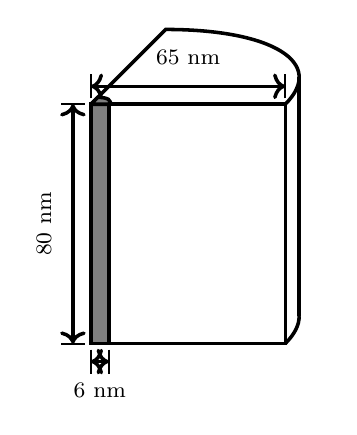
\begin{tikzpicture}[scale=0.038]

%%%%%%%%%%%%%%%%%%%%%%
%%%	 Def géométrie  %%%
%%%%%%%%%%%%%%%%%%%%%%

\def \rayonun{6}
\def \rayondeux{65}
\def \vspace{2}
\def \lignecote{8}
\def \hauteur{80}
\def \anglearc{111.5}

%%%%%%%%%%%%%%%%%%%%%%
%%%	   Def style    %%%
%%%%%%%%%%%%%%%%%%%%%%

\def \heavy{0.045cm}
\def \light{0.025cm}

%%%%%%%%%%%%%%%%%%%%%%
%%%	    Calculs     %%%
%%%%%%%%%%%%%%%%%%%%%%

\pgfmathsetmacro{\sinangle}{sin(\anglearc)}
\pgfmathsetmacro{\cosangle}{cos(\anglearc)}

%%%%%%%%%%%%%%%%%%%%%%
%%%	    Dessin      %%%
%%%%%%%%%%%%%%%%%%%%%%

\draw[line width=\heavy] (\rayonun,0) rectangle (\rayondeux,\hauteur);
\draw[line width=\heavy, fill=gray] (0,0) rectangle (\rayonun,\hauteur);
%\draw[line width=\heavy] \draw (0,0,0) arc (0:45:1) ;

% On se positionne sur un plan à une hauteur de 80 (\hauteur)
\begin{scope}[canvas is zx plane at y=\hauteur]
	% On dessine le quart de cercle extérieur
	\draw[line width=\heavy] (0,\rayondeux) arc (90:180:\rayondeux) -- (0,0);
	% On dessine le quart de cercle du nanotube
	\draw[line width=\heavy, fill=gray] (0,0) -- (0,\rayonun) arc (90:180:\rayonun) -- (0,0);
\end{scope}

% On se positionne sur un plan à une hauteur de 0
\begin{scope}[canvas is zx plane at y=0]
	% On trace le cercle jusqu'à l'angle \anglearc trouvé itérativement
	\draw[line width=\heavy] (0,\rayondeux) arc (90:\anglearc:\rayondeux);
\end{scope}

% Ligne du côté du cylindre
\draw[line width=\heavy] (\sinangle*\rayondeux,0,\cosangle*\rayondeux) -- +(0,\hauteur,0);

%%%%%%%%%%%%%%%%%%%%%%
%%%	    Cotation    %%%
%%%%%%%%%%%%%%%%%%%%%%

% On dessine la ligne de cote pour la nanotube
\draw[line width=\light] (0,-\vspace) -- + (0,-\lignecote);
\draw[line width=\light] (\rayonun,-\vspace) -- + (0,-\lignecote);
\draw[<->,line width=\heavy] (0,-\vspace-0.5*\lignecote) -- + (\rayonun,0);

\node[anchor=north] (A) at (0.5*\rayonun , -\vspace-\lignecote) {\footnotesize \rayonun \ nm};

% On dessine la ligne de cote pour la hauteur
\draw[line width=\light] (-\vspace,0) -- + (-\lignecote,0);
\draw[line width=\light] (-\vspace,\hauteur) -- + (-\lignecote,0);
\draw[<->,line width=\heavy] (-\vspace-0.5*\lignecote,0) -- + (0,\hauteur);

\node[anchor=south, rotate=90] (A) at (-\vspace-\lignecote,0.5*\hauteur ) {\footnotesize \hauteur \ nm};

% On dessine la ligne de cote pour le diamètre du modèle
\draw[line width=\light] (0,\hauteur+\vspace) -- + (0,\lignecote);
\draw[line width=\light] (\rayondeux,\hauteur+\vspace) -- + (0,\lignecote);
\draw[<->,line width=\heavy] (0,\hauteur+\vspace+0.5*\lignecote) -- + (\rayondeux,0);

\node[anchor=south] (A) at (0.5*\rayondeux , \hauteur+\vspace+\lignecote) {\footnotesize \rayondeux \ nm};

%%%%%%%%%%%%%%%%%%%%%%%%%%%%%%%%%%%%%%%%%

\end{tikzpicture}

%\shorthandon{:!}
		%}
		\caption{Quarter view of the revolved 2D axisymmetric FEM simulating the Joule heating within a MWCNT}
		\label{fig:geometry_axisymmetric}
	\end{subfigure}%
	\begin{subfigure}{55mm}
		\center
		\captionsetup{width=50mm}
		%\resizebox{65mm}{!}{
		\includegraphics[width=50mm]{geometry_3D}
		%\tikzsetnextfilename{geometry_3D}
		%%\shorthandoff{:!}

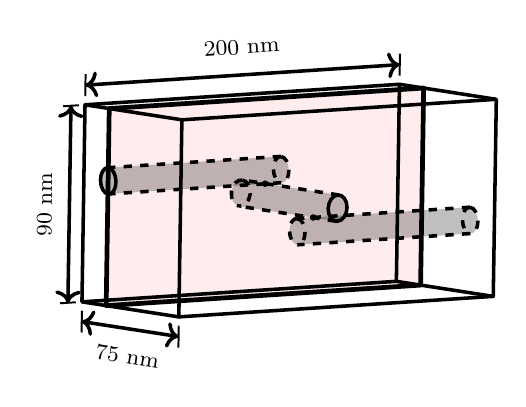
\begin{tikzpicture}[scale=0.02,
								x  = {(0.99788,0.065079)},
                    		y  = {(0.021693,1.38835)},
                    		z  = {(-0.824336,0.130158)},]

%%%%%%%%%%%%%%%%%%%%%%
%%%	 Def géométrie  %%%
%%%%%%%%%%%%%%%%%%%%%%

\def \dia{6} %La variable dia contient en fait le rayon des tubes au lieu du diamètre
\def \epaisseur{75}
\def \hauteur{90}
\def \longueur{200}

\def \angle{88.0}

\def \vspace{4}
\def \lignecote{10}
\def \anglearc{111.5}

\def \colplan{red!7}
\def \coltube{gray!50}

\def \dotsize{60pt}

\coordinate (A) at (0,0,0);
\coordinate (B) at (0,0,\epaisseur);
\coordinate (C) at (0,\hauteur,\epaisseur);
\coordinate (D) at (0,\hauteur,0);
\coordinate (E) at (-\longueur,0,0);
\coordinate (F) at (-\longueur,0,\epaisseur);
\coordinate (G) at (-\longueur,\hauteur,\epaisseur);
\coordinate (H) at (-\longueur,\hauteur,0);

\coordinate (W) at (0,0,0.75*\epaisseur);
\coordinate (X) at (0,\hauteur,0.75*\epaisseur);
\coordinate (Y) at (-\longueur,\hauteur,0.75*\epaisseur);
\coordinate (Z) at (-\longueur,0,0.75*\epaisseur);


%%%%%%%%%%%%%%%%%%%%%%
%%%	   Def style    %%%
%%%%%%%%%%%%%%%%%%%%%%

\def \heavy{0.045cm}
\def \light{0.025cm}
\def \reallyheavy{0.06cm}

%Modification du monde de transparence pour mélanger les couleurs superposées
\begin{scope}[blend mode=multiply]

%%%%%%%%%%%%%%%%%%%%%%
%%%	    Calculs     %%%
%%%%%%%%%%%%%%%%%%%%%%

\pgfmathsetmacro{\sinangle}{sin(\anglearc)}
\pgfmathsetmacro{\cosangle}{cos(\anglearc)}

\pgfmathsetmacro{\sinangledeux}{sin(\angle)}
\pgfmathsetmacro{\cosangledeux}{cos(\angle)}

%%%%%%%%%%%%%%%%%%%%%%
%%%	 Dessin du cube %%%
%%%%%%%%%%%%%%%%%%%%%%

\draw[line width=\heavy, line join=round] (A) -- (B) -- (C) --(D) -- cycle;
\draw[line width=\heavy, line join=round] (E) -- (F) -- (G) --(H) -- cycle;
\draw[line width=\heavy, line join=round] (D) -- (H);
\draw[line width=\heavy, line join=round] (G) -- (C);
\draw[line width=\heavy, line join=round] (A) -- (E);
\draw[line width=\heavy, line join=round] (F) -- (B);


%%%%%%%%%%%%%%%%%%%%%%%%%%%%%%%%%%%%
%%% Dessin du nanotube du centre %%%
%%%%%%%%%%%%%%%%%%%%%%%%%%%%%%%%%%%%

%Trouver les distances projetées en x et y pour un vecteur unitaire pour chaque axe
\path (1,0,0);
\pgfgetlastxy{\cylxx}{\cylxy}
\path (0,1,0);
\pgfgetlastxy{\cylyx}{\cylyy}
\path (0,0,1);
\pgfgetlastxy{\cylzx}{\cylzy}

%Calculs
\pgfmathsetmacro{\cylt}{(\cylzy * \cylyx - \cylzx * \cylyy)/ (\cylzy * \cylxx - \cylzx * \cylxy)}
\pgfmathsetmacro{\ang}{atan(\cylt)}
\pgfmathsetmacro{\ct}{1/sqrt(1 + (\cylt)^2)}
\pgfmathsetmacro{\st}{\cylt * \ct}

%\node[anchor=north] (A) at (0,-30,0) {\large xx \cylxx};
%\node[anchor=north] (A) at (0,-40,0) {\large xy \cylxy};
%\node[anchor=north] (A) at (0,-50,0) {\large yx \cylyx};
%\node[anchor=north] (A) at (0,-60,0) {\large yy \cylyy};
%\node[anchor=north] (A) at (0,-70,0) {\large zx \cylzx};
%\node[anchor=north] (A) at (0,-80,0) {\large zy \cylzy};
%\node[anchor=north] (A) at (0,-90,0) {\large \cylt};
%\node[anchor=north] (A) at (0,-100,0) {\large \ang};
%\node[anchor=north] (A) at (0,-110,0) {\large \ct};
%\node[anchor=north] (A) at (0,-120,0) {\large \st};

%\draw[line width=0.45, line join=round] (A) -- (H);

%Surface extérieure du cylindre
\fill[\coltube] (-0.5*\longueur+\dia*\ct,0.5*\hauteur+\dia*\st,\epaisseur) -> ++(0,0,-\epaisseur) arc[start angle=\ang,delta angle=180,radius=\dia] -- ++(0,0,\epaisseur) arc[start angle=\ang+180,delta angle=-180,radius=\dia];

%Lignes des côtés
\begin{scope}[every path/.style={line width=\heavy}]

	%Cercle du devant
	\draw[fill=\coltube] (-0.5*\longueur,0.5*\hauteur,0) circle[radius=\dia];

	%Ligne des côtés
	\draw[dashed] (-0.5*\longueur+\dia*\ct,0.5*\hauteur+\dia*\st,0) -- ++(0,0,\epaisseur);
	\draw[dashed] (-0.5*\longueur-\dia*\ct,0.5*\hauteur-\dia*\st,0) -- ++(0,0,\epaisseur);

	%Cercle arrière
	\draw[dashed] (-0.5*\longueur+\dia*\ct,0.5*\hauteur+\dia*\st,\epaisseur) arc[start angle=\ang,delta angle=180,radius=\dia];
	\draw[dashed] (-0.5*\longueur+\dia*\ct,0.5*\hauteur+\dia*\st,\epaisseur) arc[start angle=\ang,delta angle=-180,radius=\dia];
	
\end{scope}

%\draw (-0.5*\longueur,.5*\hauteur,0) -- (-0.5*\longueur,.5*\hauteur,\epaisseur);

%%%%%%%%%%%%%%%%%%%%%%%%%%%%%%%%%%%%
%%% Dessin du nanotube de droite %%%
%%%%%%%%%%%%%%%%%%%%%%%%%%%%%%%%%%%%

\begin{scope}[canvas is zy plane at x=0]
	\draw[line width=\heavy, dashed] (0.25*\epaisseur,0.5*\hauteur-2*\dia) ++(\angle:\dia) arc[start angle=\angle,delta angle=-180,radius=\dia];
	\draw[line width=\heavy, dashed, fill=\coltube] (0.25*\epaisseur,0.5*\hauteur-2*\dia) ++(\angle:\dia) arc[start angle=\angle,delta angle=180,radius=\dia];
\end{scope}


\begin{scope}[canvas is zy plane at x=-0.55*\longueur]
	\draw[line width=\heavy, dashed, fill=\coltube] (0.25*\epaisseur,0.5*\hauteur-2*\dia) ++(\angle:\dia) arc[start angle=\angle,delta angle=-180,radius=\dia];
	\draw[line width=\heavy, dashed] (0.25*\epaisseur,0.5*\hauteur-2*\dia) ++(\angle:\dia) arc[start angle=\angle,delta angle=180,radius=\dia];
\end{scope}


\draw[line width=\heavy, dashed] (0,0.5*\hauteur-2*\dia+\dia*\sinangledeux,0.25*\epaisseur+\dia*\cosangledeux) -- ++(-0.55*\longueur,0,0);	

\draw[line width=\heavy, dashed] (0,0.5*\hauteur-2*\dia-\dia*\sinangledeux,0.25*\epaisseur-\dia*\cosangledeux) -- ++(-0.55*\longueur,0,0);	

\fill[\coltube] (0,0.5*\hauteur-2*\dia+\dia*\sinangledeux,0.25*\epaisseur+\dia*\cosangledeux) -- ++(-0.55*\longueur,0,0) -- ++(0,-2*\dia*\sinangledeux,-2*\dia*\cosangledeux)-- ++(0.55*\longueur,0,0) -- cycle;

%\draw (0,0.5*\hauteur-\dia,\epaisseur*0.25) -- ++(-0.55*\longueur,0,0);


%%%%%%%%%%%%%%%%%%%%%%%%%%%%%%%%%%%%
%%% Dessin du nanotube de gauche %%%
%%%%%%%%%%%%%%%%%%%%%%%%%%%%%%%%%%%%


\begin{scope}[canvas is zy plane at x=-\longueur]
	\draw[line width=\heavy, fill=\coltube] (0.75*\epaisseur,0.5*\hauteur+2*\dia) ++(\angle:\dia) arc[start angle=\angle,delta angle=-180,radius=\dia];
	\draw[line width=\heavy] (0.75*\epaisseur,0.5*\hauteur+2*\dia) ++(\angle:\dia) arc[start angle=\angle,delta angle=180,radius=\dia];
\end{scope}

\begin{scope}[canvas is zy plane at x=-0.45*\longueur]
	\draw[line width=\heavy, dashed] (0.75*\epaisseur,0.5*\hauteur+2*\dia) ++(\angle:\dia) arc[start angle=\angle,delta angle=-180,radius=\dia];
	\draw[line width=\heavy, dashed, fill=\coltube] (0.75*\epaisseur,0.5*\hauteur+2*\dia) ++(\angle:\dia) arc[start angle=\angle,delta angle=180,radius=\dia];
\end{scope}

\draw[line width=\heavy, dashed] (-0.45*\longueur,0.5*\hauteur+2*\dia+\dia*\sinangledeux,0.75*\epaisseur+\dia*\cosangledeux) -- ++(-0.55*\longueur,0,0);	

\draw[line width=\heavy, dashed] (-0.45*\longueur,0.5*\hauteur+2*\dia-\dia*\sinangledeux,0.75*\epaisseur-\dia*\cosangledeux) -- ++(-0.55*\longueur,0,0);	

\fill[\coltube] (-0.45*\longueur,0.5*\hauteur+2*\dia+\dia*\sinangledeux,0.75*\epaisseur+\dia*\cosangledeux) -- ++(-0.55*\longueur,0,0) -- ++(0,-2*\dia*\sinangledeux,-2*\dia*\cosangledeux)-- ++(0.55*\longueur,0,0) -- cycle;

%%%%%%%%%%%%%%%%%%%%%%%%%%%%%%%%%%%%
%%% Dessin des points de contact %%%
%%%%%%%%%%%%%%%%%%%%%%%%%%%%%%%%%%%%

\fill [black] (-0.5*\longueur,0.5*\hauteur-\dia,0.25*\epaisseur) circle (\dotsize);
\fill [black] (-0.5*\longueur,0.5*\hauteur+\dia,0.75*\epaisseur) circle (\dotsize);

%%%%%%%%%%%%%%%%%%%%%%%%%%%%%%%%%%%%
%%% Dessin du plan de decoupe    %%%
%%%%%%%%%%%%%%%%%%%%%%%%%%%%%%%%%%%%

\draw[line width=\reallyheavy, line join=round, fill=\colplan] (W) -- (X) -- (Y) --(Z) -- cycle;

%%%%%%%%%%%%%%%%%%%%%%
%%%	    Cotation    %%%
%%%%%%%%%%%%%%%%%%%%%%

%Calcul des angles de rotation pour les cotes
\pgfmathsetmacro{\rotx}{ atan( \cylxy / \cylxx) }
\pgfmathsetmacro{\roty}{ atan( \cylyx / \cylyy) }
\pgfmathsetmacro{\rotz}{ atan( \cylzy / \cylzx) }

% On dessine la ligne de cote pour la longueur
\draw[line width=\light] (-\longueur,\vspace+\hauteur,\epaisseur) -- + (0,\lignecote,0);
\draw[line width=\light] (0,\vspace+\hauteur,\epaisseur) -- + (0,\lignecote,0);
\draw[<->,line width=\heavy] (-\longueur,+\vspace+\hauteur+0.5*\lignecote,\epaisseur) -- + (\longueur,0,0);

\node[anchor=south, rotate=\rotx] (C) at (-0.5*\longueur,\hauteur+\vspace+\lignecote,\epaisseur ) {\footnotesize \longueur \ nm};

% On dessine la ligne de cote pour la hauteur
\draw[line width=\light] (-\longueur-\vspace,0,\epaisseur) -- + (-\lignecote,0,0);
\draw[line width=\light] (-\longueur-\vspace,\hauteur,\epaisseur) -- + (-\lignecote,0);
\draw[<->,line width=\heavy] (-\longueur-\vspace-0.5*\lignecote,0,\epaisseur) -- + (0,\hauteur);

\node[anchor=south, rotate=90-\roty] (C) at (-\longueur-\vspace-\lignecote,0.5*\hauteur,\epaisseur ) {\footnotesize \hauteur \ nm};

% On dessine la ligne de cote pour l'épaisseur
\draw[line width=\light] (-\longueur,-\vspace,\epaisseur) -- + (0,-\lignecote,0);
\draw[line width=\light] (-\longueur,-\vspace,0) -- + (0,-\lignecote,0);
\draw[<->,line width=\heavy] (-\longueur,-\vspace-0.5*\lignecote,\epaisseur) -- + (0,0,-\epaisseur);

\node[anchor=north, rotate=\rotz] (C) at (-\longueur,-\vspace-\lignecote,0.5*\epaisseur ) {\footnotesize \epaisseur \ nm};

\end{scope}

\end{tikzpicture}

%\shorthandon{:!}
		%}
		\caption{Geometry of the second FEM evaluating the effect of charge concentration at contact point}
		\label{fig:geometry_3D}
	\end{subfigure}
	\begin{subfigure}{40mm}
		\center
		\captionsetup{width=40mm}
		%\resizebox{35mm}{!}{
		\includegraphics[width=40mm]{geometry_gap}
		%\tikzsetnextfilename{geometry_gap}
		%%\shorthandoff{:!}

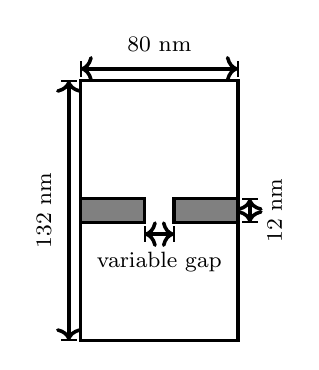
\begin{tikzpicture}[scale=0.025]

%%%%%%%%%%%%%%%%%%%%%%
%%%	 Def géométrie  %%%
%%%%%%%%%%%%%%%%%%%%%%

\def \diacnt{12}
\def \longueur{80}
\def \vspace{2}
\def \lignecote{8}
\def \hauteur{132}
\def \anglearc{111.5}
\def \gap{15}

%%%%%%%%%%%%%%%%%%%%%%
%%%	   Def style    %%%
%%%%%%%%%%%%%%%%%%%%%%

\def \heavy{0.045cm}
\def \light{0.025cm}

%%%%%%%%%%%%%%%%%%%%%%
%%%	    Calculs     %%%
%%%%%%%%%%%%%%%%%%%%%%

\pgfmathsetmacro{\sinangle}{sin(\anglearc)}
\pgfmathsetmacro{\cosangle}{cos(\anglearc)}

%%%%%%%%%%%%%%%%%%%%%%
%%%	    Dessin      %%%
%%%%%%%%%%%%%%%%%%%%%%

\draw[line width=\heavy] (0,0) rectangle (\longueur,\hauteur);
\draw[line width=\heavy, fill=gray] (0,0.5*\hauteur-0.5*\diacnt) rectangle (0.5*\longueur-0.5*\gap,0.5*\hauteur+0.5*\diacnt);
\draw[line width=\heavy, fill=gray] (0.5*\longueur+0.5*\gap,0.5*\hauteur-0.5*\diacnt) rectangle (\longueur,0.5*\hauteur+0.5*\diacnt);


%%%%%%%%%%%%%%%%%%%%%%
%%%	    Cotation    %%%
%%%%%%%%%%%%%%%%%%%%%%

% On dessine la ligne de cote pour l'espace entre les nanotubes
\draw[line width=\light] (0.5*\longueur-0.5*\gap,-\vspace+0.5*\hauteur-0.5*\diacnt) -- + (0,-\lignecote);
\draw[line width=\light] (0.5*\longueur+0.5*\gap,-\vspace+0.5*\hauteur-0.5*\diacnt) -- + (0,-\lignecote);
\draw[<->,line width=\heavy] (0.5*\longueur-0.5*\gap,-\vspace-0.5*\lignecote+0.5*\hauteur-0.5*\diacnt) -- + (\gap,0);

\node[anchor=north] (A) at (0.5*\longueur , -\vspace-\lignecote+0.5*\hauteur-0.5*\diacnt) {\footnotesize variable gap};

% On dessine la ligne de cote pour le diamètre des nanotubes
\draw[line width=\light] (\longueur+\vspace,0.5*\hauteur-0.5*\diacnt) -- + (\lignecote,0);
\draw[line width=\light] (\longueur+\vspace,0.5*\hauteur+0.5*\diacnt) -- + (\lignecote,0);
\draw[<->,line width=\heavy] (\longueur+\vspace+0.5*\lignecote,0.5*\hauteur-0.5*\diacnt) -- + (0,\diacnt);

\node[anchor=north, rotate=90] (B) at (\longueur+\vspace+\lignecote,0.5*\hauteur ) {\footnotesize \diacnt \ nm};

% On dessine la ligne de cote pour la hauteur
\draw[line width=\light] (-\vspace,0) -- + (-\lignecote,0);
\draw[line width=\light] (-\vspace,\hauteur) -- + (-\lignecote,0);
\draw[<->,line width=\heavy] (-\vspace-0.5*\lignecote,0) -- + (0,\hauteur);

\node[anchor=south, rotate=90] (C) at (-\vspace-\lignecote,0.5*\hauteur ) {\footnotesize \hauteur \ nm};

% On dessine la ligne de cote pour le diamètre du modèle
\draw[line width=\light] (0,\hauteur+\vspace) -- + (0,\lignecote);
\draw[line width=\light] (\longueur,\hauteur+\vspace) -- + (0,\lignecote);
\draw[<->,line width=\heavy] (0,\hauteur+\vspace+0.5*\lignecote) -- + (\longueur,0);

\node[anchor=south] (D) at (0.5*\longueur , \hauteur+\vspace+\lignecote) {\footnotesize \longueur \ nm};

%%%%%%%%%%%%%%%%%%%%%%%%%%%%%%%%%%%%%%%%%

\end{tikzpicture}

%\shorthandon{:!}
		%}
		\caption{Geometry of the third FEM simulating Joule heating within the polymer matrix}
		\label{fig:geometry_gap}
	\end{subfigure} 
	\caption{Geometries of the representative elementary volume composed of MWCNT (dark region) and the insulating matrix (white region) \cite{Brassard2018_REV}}
	\label{fig:geometry}
\end{figure}

\begin{figure}[htb]
	\centering
	\captionsetup{width=125mm}
	\begin{subfigure}{65mm}
		\centering
		\captionsetup{width=65mm}
		\includegraphics[width=65mm]{beamer_IC3_DBrassard-figure1.pdf}
		\caption{Resistance welding main components \cite{Brassard2018_welding_schematic}}
		\label{fig:welding_jig_schematic}
	\end{subfigure}
	\begin{subfigure}{55mm}
		\centering
		\captionsetup{width=55mm}
		\includegraphics[width=55mm]{20161026_152818_resize.jpg}
		\caption{Ceramic insulators, copper electrodes and load cell}
		\label{fig:welding_jig_electrodes}
	\end{subfigure}%	
	\caption{Resistance welding jig}
	\label{fig:welding_jig}
\end{figure}

\begin{figure}
		\center
		\captionsetup{width=60mm}
		%\resizebox{60mm}{!}{
		\includegraphics[width=60mm]{thermocouple_welding}
		%\tikzsetnextfilename{thermocouple_welding}
		%\usetikzlibrary{arrows.meta,shapes,positioning,shadows,trees,decorations.pathmorphing}

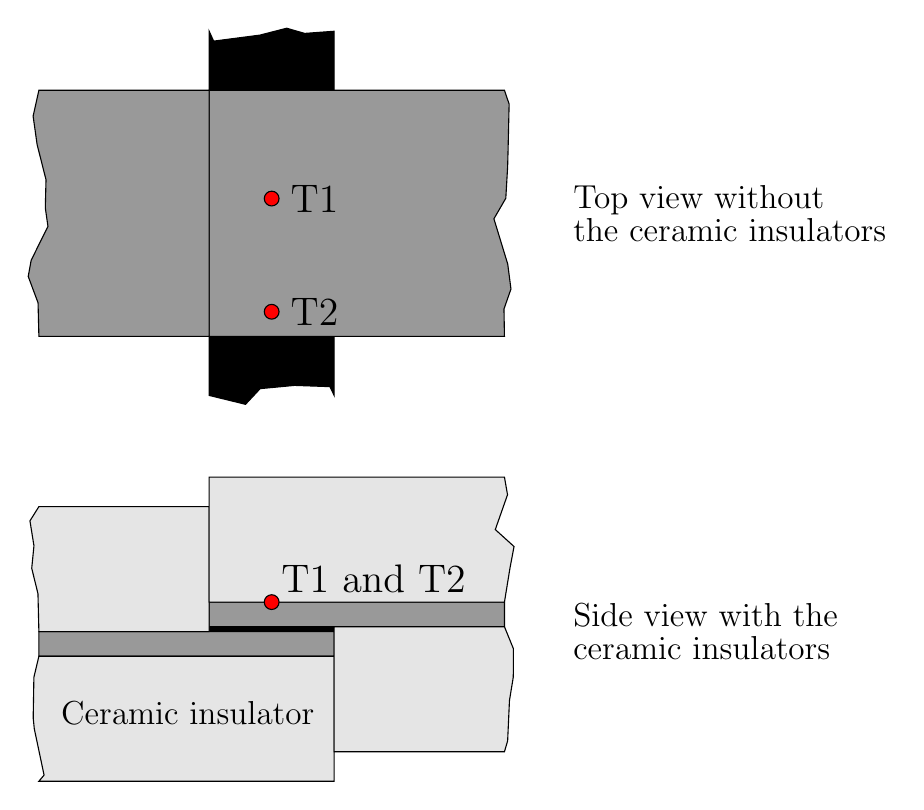
\begin{tikzpicture}[scale=0.125]

%Couleurs
\def \colceramique{black!10}
\def \colcomposite{black!40}

%Définition des dimensions du joint soudé
\def \overlap{12.7}
\def \epceramique{12.7}
\def \epcomposite{2.5}
\def \epnanocomposite{0.5}
\def \longueur{30}
\def \gapfigure{30}
\def \largeursoudure{25}
\def \depassementsoudure{6}
\def \diacercle{0.75}

%%%Vue du dessus %%%
\draw (\longueur+\depassementsoudure,\gapfigure+0.5*\largeursoudure) node [right, align=left]{\large Top view without \\ \large the ceramic insulators};

%Élément chauffant
\draw[black,decoration={random steps, amplitude=4, segment length=10},fill=black] (0,\gapfigure-\depassementsoudure) decorate{-- ++(\overlap,0)} -- ++(0,2*\depassementsoudure+\largeursoudure) decorate{-- ++(-\overlap,0)} -- cycle;

%Adhérent
\draw[black,decoration={random steps, amplitude=4, segment length=10},fill=\colcomposite] 
(0,\gapfigure) -- ++(\longueur,0) decorate{-- ++(0,\largeursoudure)} -- ++(-\longueur,0) -- cycle;
\draw[black,decoration={random steps, amplitude=4, segment length=10},fill=\colcomposite] 
(0,\gapfigure) -- ++(-\longueur+\overlap,0) decorate{-- ++(0,\largeursoudure)} -- ++(\longueur-\overlap,0) -- cycle;

%Position du thermocouple
\draw[fill=red] (0.5*\overlap,\gapfigure+14) circle (0.75) node [right]{\ \Large T1};
\draw[fill=red] (0.5*\overlap,\gapfigure+2.5) circle (0.75) node [right]{\ \Large T2};


%%% Vue du côté %%%
\draw (\longueur+\depassementsoudure,0) node [right, align=left]{\large Side view with the \\ \large ceramic insulators};

%Éléments chauffants
\draw[black,thick,fill=black] (0,0) -- ++(\overlap,0) -- ++(0,\epnanocomposite) -- ++(-\overlap,0) -- cycle;

%Adhérents
\draw[black,decoration={random steps, amplitude=4, segment length=6},fill=\colcomposite] 
(\overlap,0) -- ++(-\longueur,0) decorate{-- ++(0,-\epcomposite)} -- ++(\longueur,0) -- cycle;
\draw[black,decoration={random steps, amplitude=4, segment length=6},fill=\colcomposite] 
(0,\epnanocomposite) -- ++(\longueur,0) decorate{-- ++(0,\epcomposite)} -- ++(-\longueur,0) -- cycle;

%Céramiques
\draw[black,decoration={random steps, amplitude=4, segment length=10},fill=\colceramique] 
(\overlap,-\epcomposite) -- ++(-\longueur,0) decorate{-- ++(0,-\epceramique)} -- ++(\longueur,0) -- cycle;
\draw[black,decoration={random steps, amplitude=4, segment length=10},fill=\colceramique] 
(0,0) -- ++(-\longueur+\overlap,0) decorate{-- ++(0,\epceramique)} -- ++(\longueur-\overlap,0) -- cycle;
\draw[black,decoration={random steps, amplitude=4, segment length=10},fill=\colceramique] 
(\overlap,\epnanocomposite) -- ++(\longueur-\overlap,0) decorate{-- ++(0,-\epceramique)} -- ++(-\longueur+\overlap,0) -- cycle;
\draw[black,decoration={random steps, amplitude=4, segment length=10},fill=\colceramique] 
(0,\epnanocomposite+\epcomposite) -- ++(\longueur,0) decorate{-- ++(0,\epceramique)} -- ++(-\longueur,0) -- cycle;

%Identification des céramiques
\draw (-\longueur+1.1*\overlap,-0.65*\epceramique) node [right, align=left]{ \large Ceramic insulator};

%Position du thermocouple
\draw[fill=red] (0.5*\overlap,\epnanocomposite+\epcomposite) circle (0.75) node [above right]{\Large T1 and T2};


\end{tikzpicture}

		%}
		\caption{Location of the thermocouples during the welding process}
		\label{fig:location_thermocouple}
\end{figure} 

\begin{figure}[htb]
	\centering
	\captionsetup{width=125mm}
	\begin{subfigure}{60mm}
		\centering
		\captionsetup{width=75mm}
		\includegraphics[width=3.25in]{resultats_comsol_axisymetrique_temp}
		\caption{Temperature field}
		\label{fig:temp_axysymmetric}
	\end{subfigure}
	\begin{subfigure}{80mm}
		\centering
		\captionsetup{width=75mm}
		\includegraphics[width=3.25in]{resultats_comsol_axisymetrique_puissance}
		\caption{Heat generation field}
		\label{fig:heat_axysymmetric}
	\end{subfigure}%	
	\caption{Results of the FEM evaluating the heat generation within the MWCNT}
	\label{fig:results_axysymmetric}
\end{figure}

\begin{figure}[htb]
	\centering
	\captionsetup{width=125mm}
	\begin{subfigure}{60mm}
		\centering
		\captionsetup{width=75mm}
		\includegraphics[width=80mm]{resultats_comsol_3D_temp}
		\caption{Temperature field}
		\label{fig:temp_3D}
	\end{subfigure}
	\begin{subfigure}{80mm}
		\centering
		\captionsetup{width=75mm}
		\includegraphics[width=80mm]{resultats_comsol_3D_puissance_log}
		\caption{Heat generation field}
		\label{fig:heat_3D}
	\end{subfigure}
	\caption{Results of the FEM evaluating the effect of charge concentration and contact resistance}
	\label{fig:results_3D}
\end{figure}

\begin{figure}[htb]
	\centering
	\begin{subfigure}{60mm}
		\centering
		\captionsetup{width=55mm}
		\includegraphics[width=60mm]{resultats_0,1nm_comsol_2D_puissance}
		\caption{\SI{0.1}{\nano\metre} gap, \SI{3.1e9}{\volt\per\metre}}
		\label{fig:result_gap01nm_power}		
	\end{subfigure} 
	\begin{subfigure}{60mm}
		\centering
		\captionsetup{width=55mm}
		\includegraphics[width=60mm]{resultats_8nm_comsol_2D_puissance}
		\caption{\SI{8}{\nano\metre} gap, \SI{15e9}{\volt\per\metre}}
		\label{fig:result_gap8nm_power}		
	\end{subfigure}

	\begin{subfigure}{60mm}
		\centering
		\captionsetup{width=55mm}
		\includegraphics[width=60mm]{resultats_0,1nm_comsol_2D_temp}
		\caption{\SI{0.1}{\nano\metre} gap, \SI{3.1e9}{\volt\per\metre}}
		\label{fig:result_gap01nm_temp}		
	\end{subfigure} 
	\begin{subfigure}{60mm}
		\centering
		\captionsetup{width=55mm}
		\includegraphics[width=60mm]{resultats_8nm_comsol_2D_temp}
		\caption{\SI{8}{\nano\metre} gap, \SI{15e9}{\volt\per\metre}}
		\label{fig:result_gap8nm_temp}		
	\end{subfigure}
	\caption{Effect of the gap length on the heat generation and temperature fields in the case of heat generation within the polymer}
	\label{fig:result_gap}
\end{figure}

\begin{figure}[htb]
	\center
	\captionsetup{width=125mm}
	\begin{subfigure}{60mm}
		\center
		\captionsetup{width=50mm}
		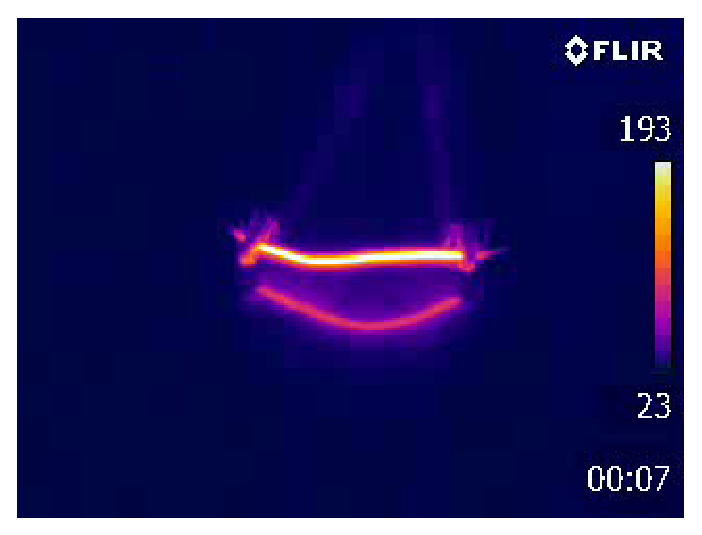
\includegraphics[width=50mm]{output0036}
		\caption{Thermographs in \si{\celsius} \cite{Brassard2018_thermograph}}
		\label{fig:results_thermal}
	\end{subfigure}
	\begin{subfigure}{80mm}
		\center
		\captionsetup{width=78mm}
		\includegraphics[width=78mm]{temperature_over_time.pdf}
		\caption{Evolution of the temperature}
		\label{fig:temp_over_time}
	\end{subfigure}%	
	\caption{Surface temperature of the polymer wire during the experiment under an AC electrical field of \SI{724}{\volt\per\metre}}
	\label{fig:results_lab}
\end{figure}

\begin{figure}[htb]
	\center
	\captionsetup{width=125mm}
	\begin{subfigure}{125mm}
		\center
		\captionsetup{width=125mm}
		\includegraphics[width=125mm]{350kW-70-10-150-1UD_crop.jpg}
		\caption{Cohesive failure with an hourglass shape in the middle and adhesive failure on the sides in a sample welded for \SI{70}{\s}}
		\label{fig:fracture_surface_70s}
	\end{subfigure}
	\begin{subfigure}{125mm}
		\center
		\captionsetup{width=125mm}
		\includegraphics[width=125mm]{350kW-90-10-150-3UD_crop.jpg}
		\caption{Mostly cohesive failure in a sample welded for \SI{90}{\s}}
		\label{fig:fracture_surface_90s}
	\end{subfigure}%	
	\caption{Fracture surface of specimens welded at \SI{350}{\kW\per\square\metre} with \SI{1.5}{\mm} clamping distance}
	\label{fig:fracture_surface}
\end{figure}

\begin{figure}[h]
	\center
	\captionsetup{width=78mm}
	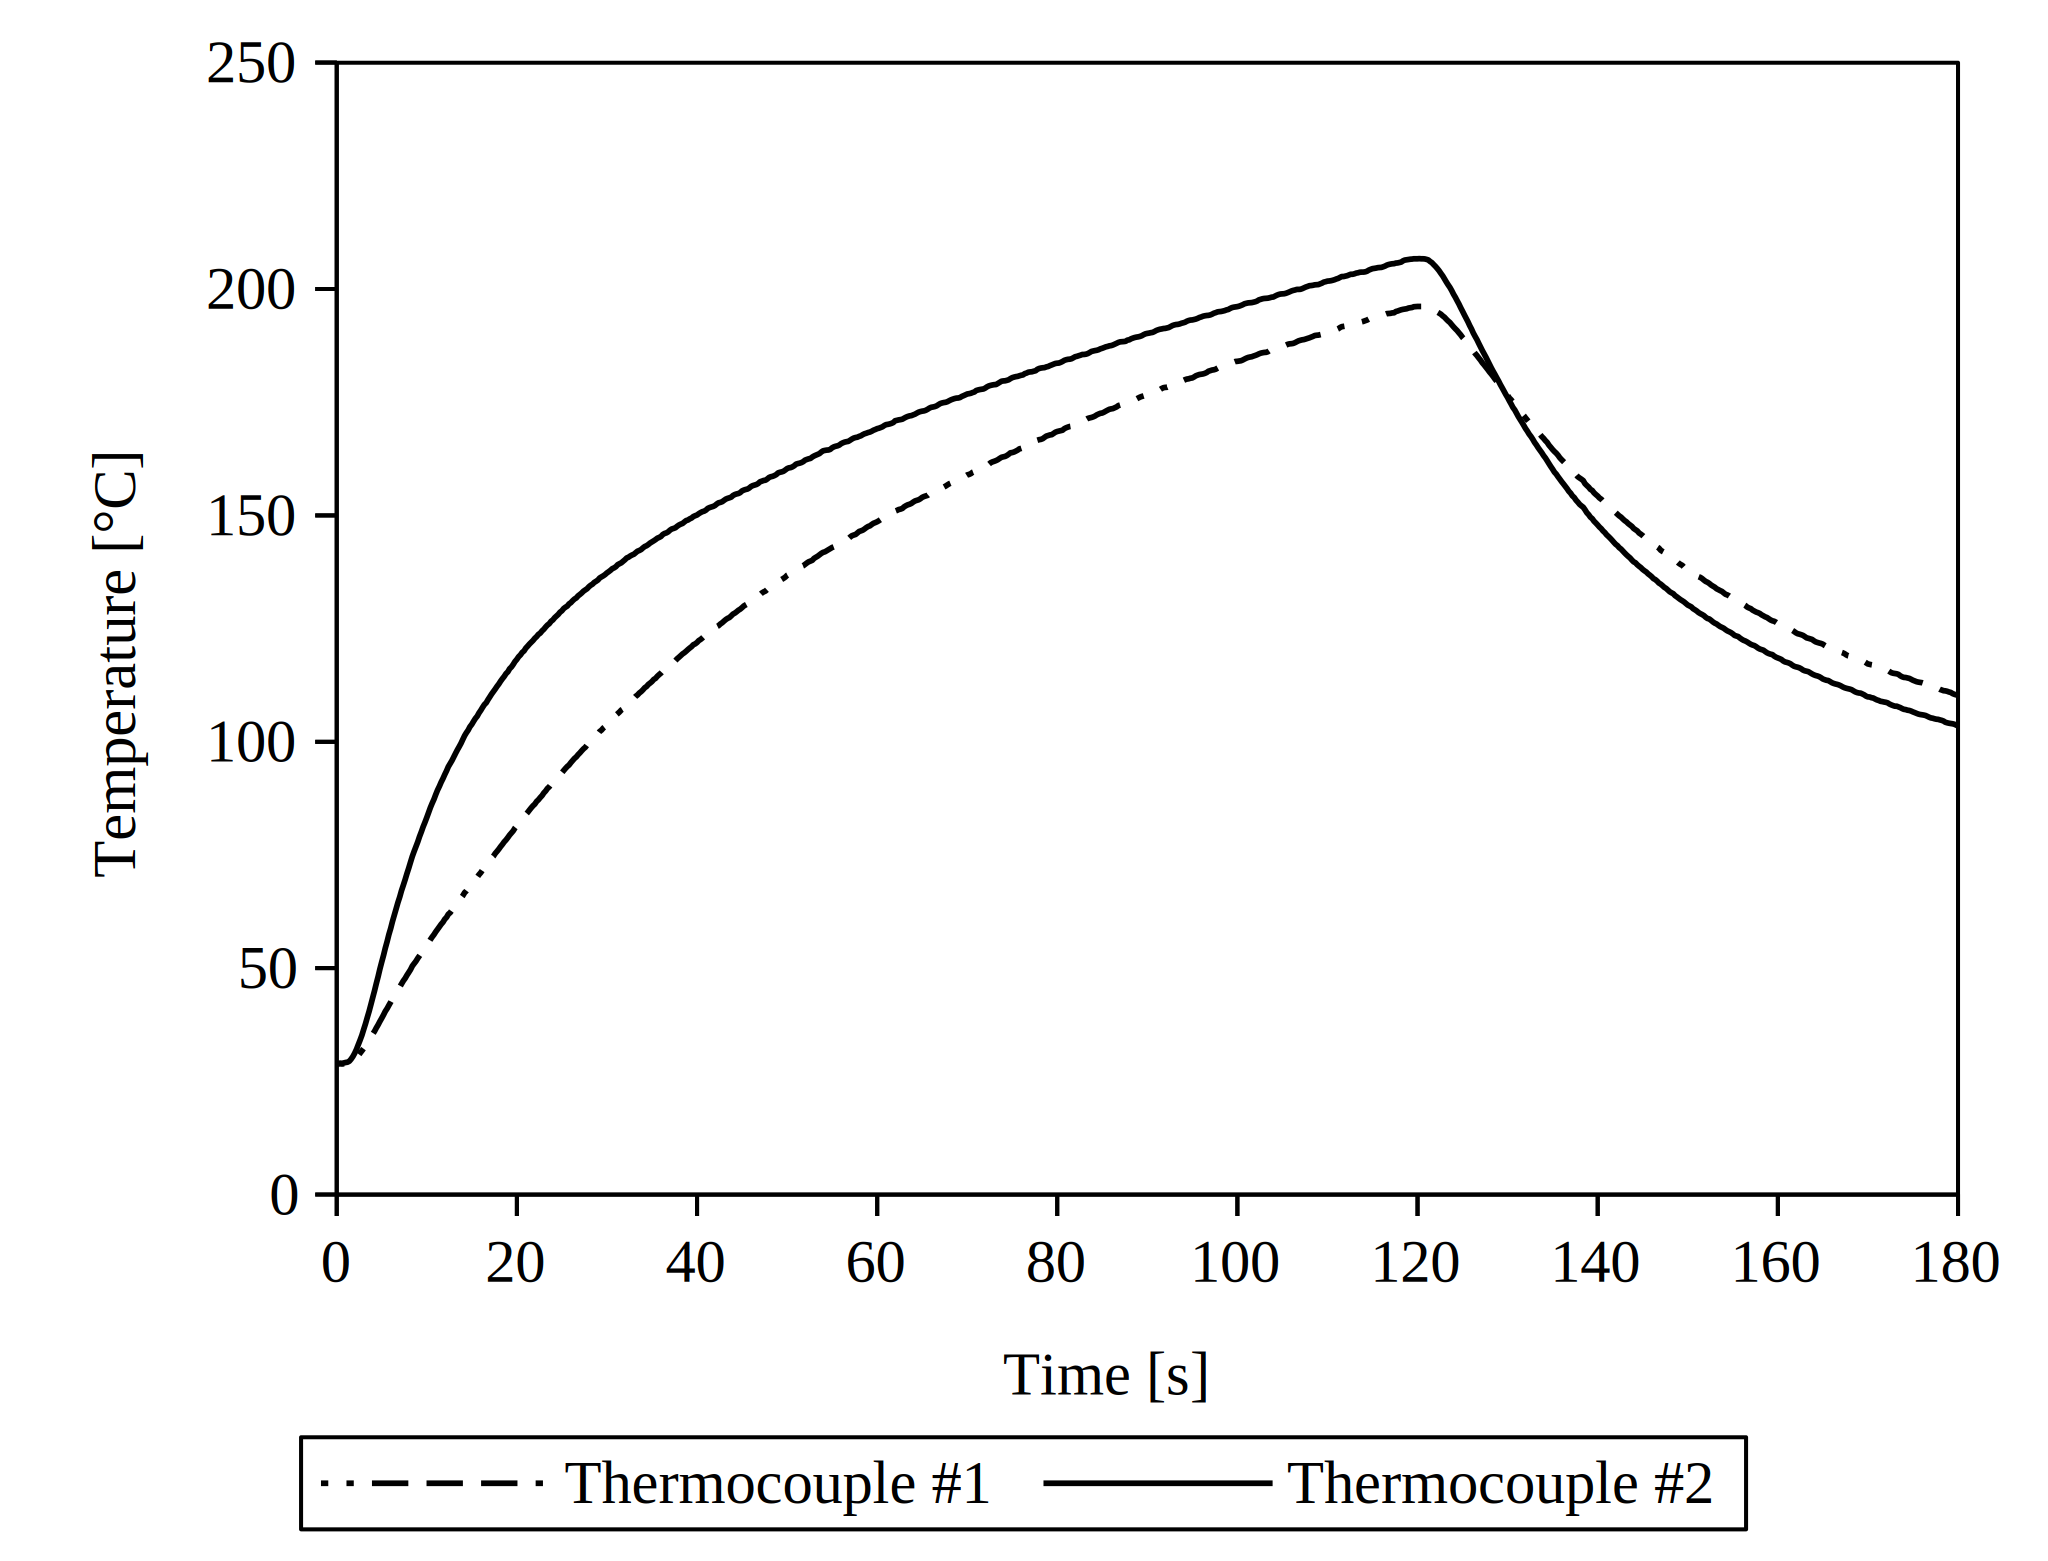
\includegraphics[width=3.25in]{temp_welding_350kw.pdf}
	\caption{Evolution of the temperature during the welding process at \SI{350}{\kilo\watt\per\square\metre} for \SI{120}{\second}}
	\label{fig:temp_350kW_120_10_150_3UD}
\end{figure}

\FloatBarrier
\clearpage
%%%%%%%%%%%%%%%%%%%%%%%%%%%%%%%%%%%%%%%%%%%%%%%%%%%%%%%%%%%%%%%%%
							\section*{Tables}
%%%%%%%%%%%%%%%%%%%%%%%%%%%%%%%%%%%%%%%%%%%%%%%%%%%%%%%%%%%%%%%%%
\FloatBarrier

\begin{table}[h]
\center
\resizebox{125mm}{!}{
\begin{tabular}{@{}lllrlrl@{}}
\toprule
Property    					&                   &        												& PEEK & 																& MWCNT 			& \\ \midrule
Density						& $\rho$            & [\si{\kilo\gram\per\cubic\metre}]  			& 1300 & \cite{cogswell1992, Giants1994}					& 2000 			& \cite{Lehman2011} \\
Specific heat				& $C_p$             & [\si{\joule\per\kilo\gram\per\celsius}] 	& 1950 & \cite{cogswell1992}									& 600 				& \cite{Mizel99} \\
Thermal conductivity		& $k$               & [\si{\watt\per\metre\per\celsius}]  			& 0.25 & \cite{cogswell1992}									& 3000				& \cite{Mizel99,Berber2000} \\
Electrical conductivity	& $\sigma$          & [\si{\siemens\per\metre}]    					& \num{2e-14} & \cite{Giants1994,Bangarusampath2009}		& \num{8.3e5}	& \cite{Ebbesen1996} \\
Relative permittivity		& $\upvarepsilon_r$ & [ \sep ]												& 3.1  &	\cite{victrexpeek, Giants1994}						& 12.5     		& \cite{Katsounaros2011} \\ \bottomrule
\end{tabular}}
\caption{Material properties}
\label{tab:material_properties}
\end{table}

\begin{table}[h]
\centering
%\resizebox{88mm}{!}{
\begin{tabular}{@{}lrrrrr@{}}
\toprule
Voltage 			& Electric					& Current 			& Maximum  					& Specific   						& Nanocomposite's \\ 
 					& field						&  						& surface 					& power   							& electrical \\ 
 					& 								&  						& temperature 				&    									& conductivity \\
{[}\si{\V}{]} 	& {[}\si{\V\per\m}{]} 	& {[}\si{\A}{]} 	& {[}\si{\celsius}{]} 	& {[}\si{\W\per\cubic\cm}{]}	& {[}\si{\siemens\per\cm}{]} \\ \midrule
10 					& 145							& 0.011 				& 24 							& 2		  								& 0.97 \\
20					& 290							& 0.031 				& 30 							& 12	 								& 1.37 \\
30 					& 435							& 0.050 				& 49 							& 28	 								& 1.48 \\
40 					& 580							& 0.073 				& 81 							& 54	 								& 1.59 \\
50 					& 724							& 0.108 				& \textgreater 150 		& 99	 								& 1.89 \\ \bottomrule
\end{tabular}%}
\caption{Electrical results from the nanocomposite filament experiments}
\label{tab:results_lab}
\end{table}

\begin{table}[H]
\centering
\resizebox{\textwidth}{!}{
\begin{tabular}{@{}lllcccc@{}}
\toprule
Clamping distance	& Values			&						& \multicolumn{4}{c}{Time}																\\
{[}\si{\mm}{]}		&					&						& \multicolumn{4}{c}{{[}\si{\s}{]}}													\\
						&					&						& 60					& 70					& 90					& 120					\\ \midrule
0						& ASS				& {[}\si{\MPa}{]}	&						&						&						& \num{14.5(13)}	\\
						& Welded area	& {[}\%{]}			&						&						&						& \num{85(2)}		\\
1						& ASS				& {[}\si{\MPa}{]}	&						&						&						& \num{13.0(44)}	\\
						& Welded area	& {[}\%{]}			&						&						& 						& \num{83(7)}		\\
1.5						& ASS				& {[}\si{\MPa}{]}	& \num{16.4(78)}	& \num{18.6(20)}	& \num{15.5(38)}	& \num{19.6(35)}	\\
						& Welded area	& {[}\%{]}			& \num{57(20)}		& \num{74(10)}		& \num{87(1)}		& \num{78(2)}		\\ \bottomrule
\end{tabular}}
\caption{ASS and fractography analysis reported as average values $\pm$ standard deviation}
\label{tab:SLS_and_fractography_results}
\end{table}


\FloatBarrier
\clearpage
%%%%%%%%%%%%%%%%%%%%%%%%%%%%%%%%%%%%%%%%%%%%%%%%%%%%%%%%%%%%%%%%%
							\section*{Supplementary Information}
%%%%%%%%%%%%%%%%%%%%%%%%%%%%%%%%%%%%%%%%%%%%%%%%%%%%%%%%%%%%%%%%%
\subsection*{Timescale analysis}
\FloatBarrier

Although PEEK has poor thermal conductivity, uniform temperature fields with temperature variations not exceeding \SI{1e-5}{\celsius} are observed in the models. 
A comparative numerical analysis of the timescales for thermal diffusion, can explain this behaviour. 
This timescale is evaluated using the time constant for thermal diffusion ($t_D$) : 

\begin{equation}
	t_D = \frac{L^2}{\alpha}
	\label{equa:time_constant}
\end{equation}

\begin{figure}[htb]
	\center
	\captionsetup{width=35mm}
	%\resizebox{35mm}{!}{%\\
	\includegraphics[width=35mm]{arrangement_carre}
	%\tikzsetnextfilename{arrangement_carre}
	%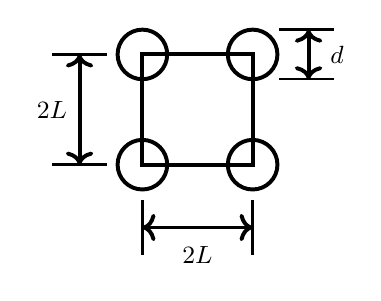
\begin{tikzpicture}[scale=1.4]

\def \l{1}
\def \r{0.225}
\def \vspace{0.32}
\def \lignecote{0.5}

\def \heavy{0.05cm}
\def \light{0.03cm}

\draw[line width=\heavy] (0,0) rectangle (\l,\l);

\draw[line width=\heavy] (0,0) circle (\r);
\draw[line width=\heavy] (\l,0) circle (\r);
\draw[line width=\heavy] (0,\l) circle (\r);
\draw[line width=\heavy] (\l,\l) circle (\r);

\draw[line width=\light] (0,-\vspace) -- + (0,-\lignecote);
\draw[line width=\light] (\l,-\vspace) -- + (0,-\lignecote);
\draw[<->,line width=\heavy] (0,-\vspace-0.5*\lignecote) -- + (\l,0);

\node (A) at (0.5*\l , -\vspace-\lignecote) {\small $2L$};

\draw[line width=\light] (-\vspace,0) -- + (-\lignecote,0);
\draw[line width=\light] (-\vspace,\l) -- + (-\lignecote,0);
\draw[<->,line width=\heavy] (-\vspace-0.5*\lignecote,0) -- + (0,\l);

\node (A) at (-\vspace-\lignecote,0.5*\l ) {\small $2L$};

\draw[line width=\light] (\l+0.75*\vspace,\l-\r) -- + (\lignecote,0);
\draw[line width=\light] (\l+0.75*\vspace,\l+\r) -- + (\lignecote,0);
\draw[<->,line width=\heavy] (\l+\vspace+0.375*\lignecote,\l-\r) -- + (0,2*\r);

\node (A) at (\l+\vspace+0.25*\lignecote+\vspace,\l ) {\small $d$};


\end{tikzpicture}
	%}
	\caption{Square packing micromechanic model}
	\label{fig:square_packing}
\end{figure}

Assuming a uniform square packing of evenly distributed particles (Fig. \ref{fig:square_packing}) of known diameter ($d$) and variable volume fractions ($v_f$), it is possible to evaluate the average half distance ($L$) between particles :

\begin{equation}
	L = \sqrt{\frac{\pi \ d^2}{16 \ v_f}}
	\label{equa:L_average}
\end{equation}

The thermal diffusivity ($\alpha$) is defined as a function of thermal conductivity ($k$), density ($\rho$) and specific heat ($C_p$) : 

\begin{equation}
	\alpha = \frac{k}{\rho \ C_p}
	\label{equa:thermal_diffusivity}
\end{equation}

\begin{table}[htb]
\centering
%\resizebox{88mm}{!}{
\begin{tabular}{@{}p{2.4cm}p{2.5cm}p{2cm}p{1.5cm}@{}}
\toprule
Weight fraction of MWCNTs	& Volume fraction of MWCNT	& Average half distance 	& \textbf{Time constant}  		\\ %\midrule
$w_f$								& $v_f$ 							& L 							& $\mathbf{t_D}$            	\\
{[}\%{]}							& {[}\%{]	}						& {[}nm{]} 					& \textbf{{[}s{]}}            	\\ \midrule
1									& 0.65 							& 65.8	 						& $\mathbf{3\times 10^{-8}}$ 	\\ 
5									& 3.31								& 29.2							& $\mathbf{6\times 10^{-9}}$	\\
10									& 6.74								& 20.5							& $\mathbf{3\times 10^{-9}}$	\\
16									& 11.02 							& 16.0 						& $\mathbf{2\times 10^{-9}}$	\\	\bottomrule
\end{tabular}%}
\caption{Timescale for heat conduction}
\label{tab:results_timescale}
\end{table}

Since the thermal conductivity of MWCNTs is very high compared to the polymer, only the properties of the matrix were considered in this timescale analysis. 
Table \ref{tab:results_timescale} presents the time constants calculated for thermal diffusion within the polymer matrix. 
The time constants varied from $3 \times 10^{-8}$ to \SI{2e-9}{\second} for $v_f$ varying from 1\% to 16\%. 
Considering that the simulations looked at Joule heating on a scale closer to the second, the short timescales for thermal diffusion explain the constant temperature fields. 

\subsection*{FTIR results}

We collected FTIR spectra from a virgin PEI pellet, a nanocomposite PEI/MWCNT pellet, a nanocomposite film and two spectra from a fracture surface of a welded zone. 
The resulting absorbances spectra were calculated. 
The appearance of characteristic peaks, their position and width remained the same between the different spectra. 

\begin{figure}[h]
	\center
	\includegraphics[width=\textwidth]{FTIR_spectra.pdf}
	\caption{Raw FTIR spectra}
	\label{fig:FTIR_spectra}
\end{figure}

\end{document}
